\section{Performance Evaluation}
\label{sec: Performance Evaluation}
This project provides a \textbf{simple demo application} for evaluating the behaviour of the \textbf{allocation algorithms} previously introduced.
The demo application can be selected by setting the \texttt{mainCREATE\_SIMPLE\_DEMO} value to \texttt{7} in the \texttt{main.c} file. 


\subsection{Demo Application}
\label{subsec: Mem Mang Demo App}
The \textbf{main} function performs the following steps:
\begin{multicols}{2} % Inizia l'ambiente a due colonne
\begin{enumerate}
    \item \textbf{Allocates 1000 bytes}
    \item \textbf{Allocates 1000 bytes}
    \item \textbf{Allocates 1500 bytes}
    \item \textbf{Allocates 100 bytes}
    \item \textbf{Allocates 100 bytes}
    \item \textbf{Allocates 100 bytes}
    \item \textbf{Allocates 100 bytes}
    \item \textbf{De-allocates 1000 bytes (second block)}
    \item \textbf{De-allocates 100 bytes (fourth block)}
    \item \textbf{De-allocates 100 bytes (fifth block)}
    \item \textbf{De-allocates 100 bytes (sixth block)}
    \item \textbf{Allocates 300 bytes}
    \item \textbf{Allocates 1000 bytes}
    \item \textbf{Creates a task (TASK 1)}
\end{enumerate}
\end{multicols}

After each operation, \textbf{the free heap space} and \textbf{the minimum ever free heap space} are recorded. If an allocation fails, the system prints an error message using the \texttt{vApplicationMallocFailedHook} function in `main.c`.

\subsection{Evaluation}
\label{subsec: Evaluation}
For this test, the heap size \texttt{(configTOTAL\_HEAP\_SIZE)} in the \texttt{FreeRTOSConfig.h} file is set to \textbf{4 kB}.

\subsubsection{First-Fit Algorithm}
When the default implementation is selected (i.e., \textbf{First-Fit}), the allocation fails before the last block of \textbf{1000 bytes} is allocated. The output obtained is shown in Table \ref{tab:firstfit}.

\begin{longtable}{|l|c|c|}
    \hline
    \textbf{Message} & \textbf{Free Heap (B)} & \textbf{Minimum Ever Free Heap (B)} \\
    \hline
    1. Before allocating memory blocks & 0 & 0 \\
    2. After allocated 1000 bytes & 3072 & 3072 \\
    3. After allocated 1000 bytes & 2064 & 2064 \\
    4. After allocated 1500 bytes & 552 & 552 \\
    5. After allocated 100 bytes & 440 & 440 \\
    6. After allocated 100 bytes & 328 & 328 \\
    7. After allocated 100 bytes & 216 & 216 \\
    8. After allocated 100 bytes & 104 & 104 \\
    9. After deallocated the second block (1000 bytes) & 1112 & 104 \\
    10. After deallocated the fourth block (100 bytes) & 1224 & 104 \\
    11. After deallocated the fifth block (100 bytes) & 1336 & 104 \\
    12. After deallocated the sixth block (100 bytes) & 1448 & 104 \\
    13. After allocated 300 bytes & 1136 & 104 \\
    \hline
    \textbf{Malloc failed..} & & \\
    \hline
    \caption{Worst-Fit Allocation Algorithm Results}
    \label{tab:firstfit}
\end{longtable}

The \textbf{heap configuration} at \textbf{step 13} (i.e., before the failure) is the following:

\begin{figure}[H]
    \centering
    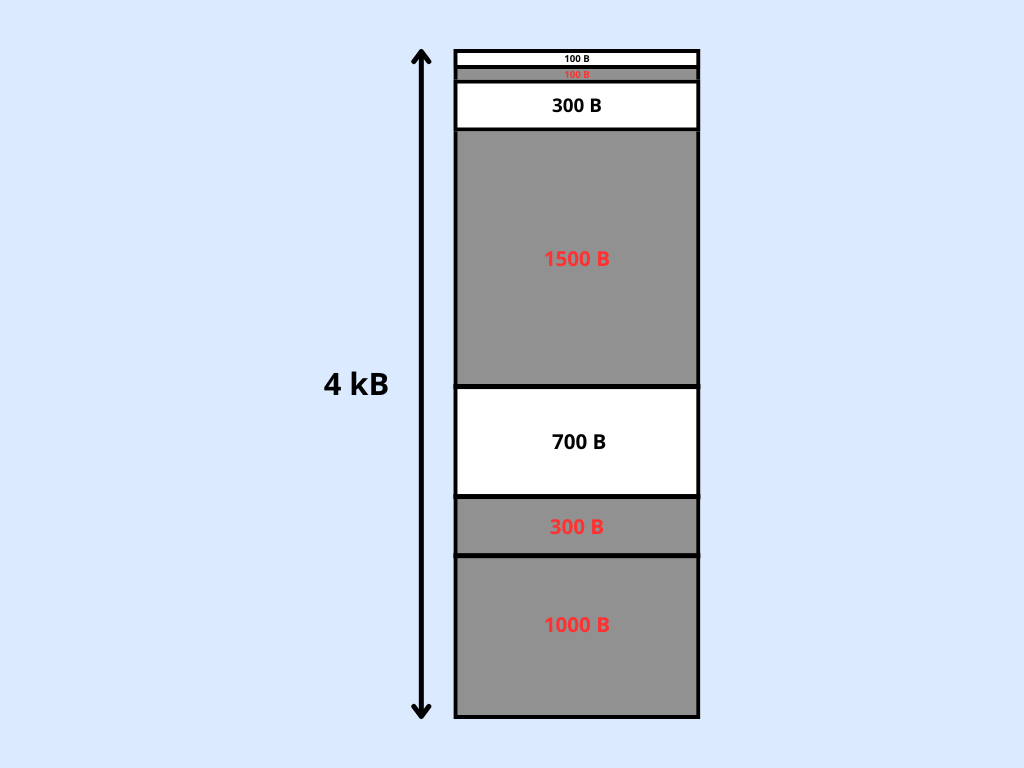
\includegraphics[width=0.5\textwidth]{img/first-worst.png}
    \caption{Heap Configuration - First-Fit}
    \label{fig:Heap Configuration - First-Fit}
\end{figure}

\newpage
\subsubsection{Best-Fit Algorithm}
When the Best-Fit algorithm is used, the system fails to allocate memory for creating the task at step 14 because there is insufficient space. The output obtained is shown in Table \ref{tab:bestfit}.
\begin{longtable}{|l|c|c|}
    \hline
    \textbf{Message} & \textbf{Free Heap (B)} & \textbf{Minimum Ever Free Heap (B)} \\
    \hline
    1. Before allocating memory blocks & 0 & 0 \\
    2. After allocated 1000 bytes & 3072 & 3072 \\
    3. After allocated 1000 bytes & 2064 & 2064 \\
    4. After allocated 1500 bytes & 552 & 552 \\
    5. After allocated 100 bytes & 440 & 440 \\
    6. After allocated 100 bytes & 328 & 328 \\
    7. After allocated 100 bytes & 216 & 216 \\
    8. After allocated 100 bytes & 104 & 104 \\
    9. After deallocated the second block (1000 bytes) & 1112 & 104 \\
    10. After deallocated the fourth block (100 bytes) & 1224 & 104 \\
    11. After deallocated the fifth block (100 bytes) & 1336 & 104 \\
    12. After deallocated the sixth block (100 bytes) & 1448 & 104 \\
    13. After allocated 300 bytes & 1136 & 104 \\
    14. After allocated 1000 bytes & 128 & 104 \\
    \hline
    \textbf{Malloc failed...} & & \\
    \hline
    \caption{Best-Fit Allocation Algorithm Results}
    \label{tab:bestfit}
\end{longtable}

At step 14, the allocation fails because there is not enough space to create the \textbf{TCB} (\textbf{Task Control Block}).
The \textbf{heap configuration} at \textbf{step 14} (i.e., before the failure) is the following:

\begin{figure}[H]
    \centering
    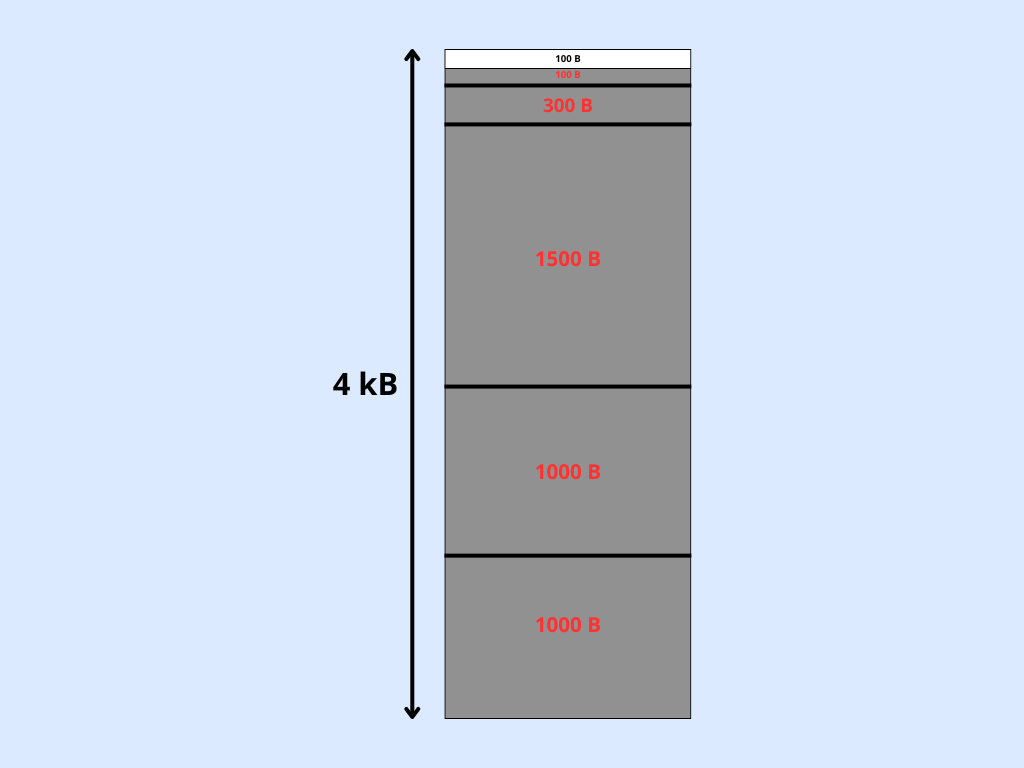
\includegraphics[width=0.5\textwidth]{img/best.png}
    \caption{Heap Configuration - Best-Fit}
    \label{fig:Heap Configuration - Best-Fit}
\end{figure}

\subsubsection{Worst-Fit Algorithm}
The output is the same obtained with \textbf{First-Fit} algorithm in Table \ref{tab:firstfit} (i.e., in this specific example the two algorithms behave in the same way). Obviously also the heap configuration before the failure is the same \ref{fig:Heap Configuration - First-Fit}.

